%!TEX root = ../main.tex

\begin{figure}[t]
\centering
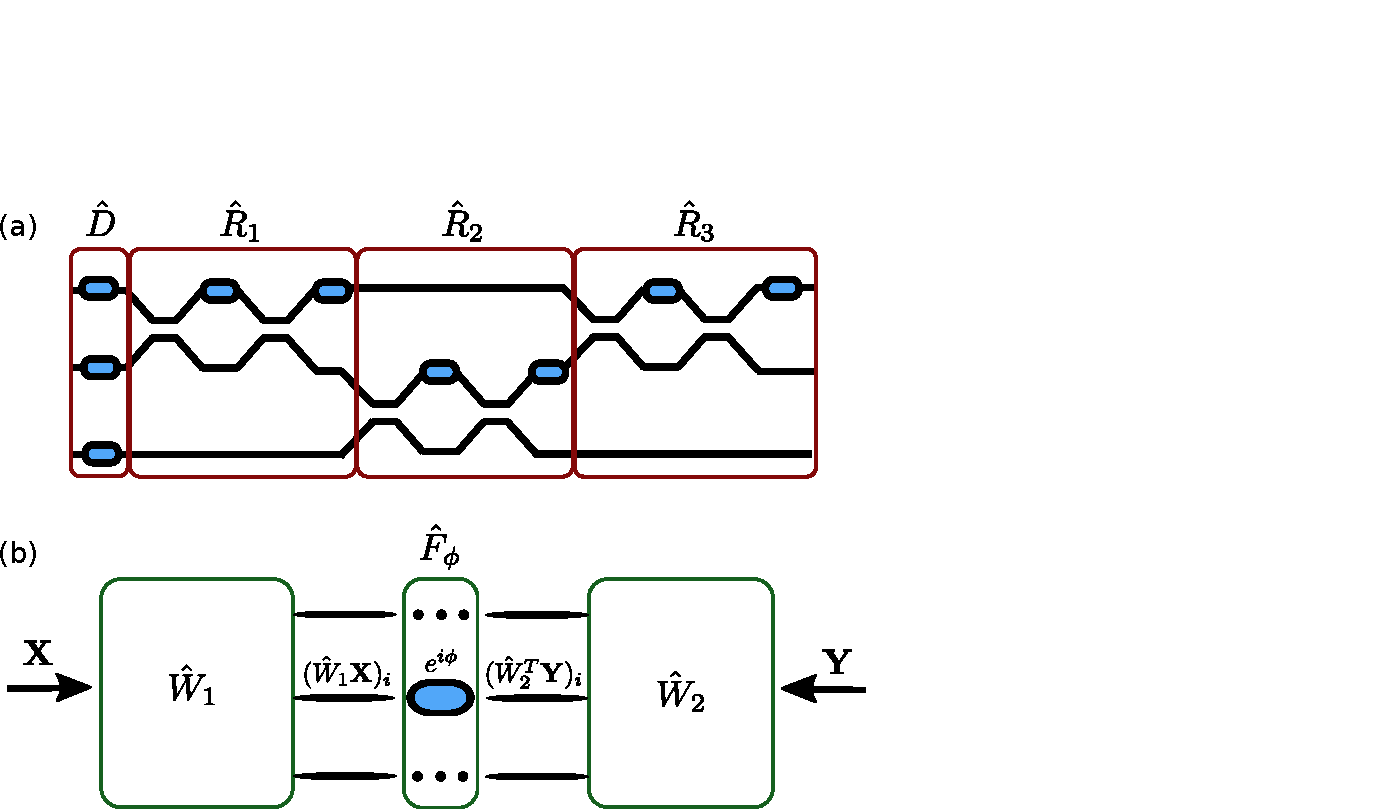
\includegraphics[width=\columnwidth, , trim = 0in 0in 3.6in 1.2in, clip = true]{figures/insitu_supp.pdf}
\caption{\label{fig:W_opt}(a): An OIU implementing a universal $3\times 3$ unitary operation, parameterized as in Ref. \cite{Clements2016}. (b): Illustration of Eq. (\ref{eqn:XY}) for the computation of the gradient with respect to a given phase shifter.}
\end{figure}

In Chapter 4 of the main text, we have shown, starting from Maxwell's equations, how the gradient information defined for an arbitrary problem can be obtained through electric field intensity measurements. However, since the full electromagnetic problem is too large to solve repeatedly, for the purposes of demonstration of a functioning neural network, in Section 6 we use the analytic, matrix representation of a mesh of MZIs as described in Ref. \cite{Clements2016}. Namely, for an even $N$, the matrix $\hat{W}$ of the OIU is parametrized as the product of $N + 1$ unitary matrices:
%
\begin{equation}
\hat{W} = \hat{R}_N \hat{R}_{N-1} \dots \hat{R}_2 \hat{R}_1 \hat{D} ,
\label{eq:W_R}
\end{equation}
%
where each $\hat{R}_i$ implements a number of two-by-two unitary operations corresponding to a given MZI, and $\hat{D}$ is a diagonal matrix corresponding to an arbitrary phase delay added to each port. This is schematically illustrated in Fig. \ref{fig:W_opt}(a) for $N = 3$. For the ANN training, we need to compute terms of the form 
%
\begin{equation}
\frac{d\mathcal{L}}{d\phi} =
\mathcal{R}\left\{ \mathbf{Y}^T \frac{d \hat{W}}{d\phi} \mathbf{X} \right\},
\label{eqn:L}
\end{equation}
%
for an arbitrary phase $\phi$ and vectors $\mathbf{X}$ and $\mathbf{Y}$ defined following the steps in the main text. Because of the feed-forward nature of the OIU-s, the matrix $\hat{W}$ can also be split as
%
\begin{equation}
\hat{W} = \hat{W}_2 \hat{F_\phi} \hat{W}_1,
\end{equation}
%
where $\hat{F_\phi}$ is a diagonal matrix which applies a phase shift $e^{i\phi}$ in port $i$ (the other elements are independent of $\phi$), while $\hat{W}_1$ and $\hat{W}_2$ are the parts that precede and follow the phase shifter, respectively (Fig. \ref{fig:W_opt}(b)). Thus, Eq. (\ref{eqn:L}) becomes 
%
\begin{align}
\mathcal{R}\left\{ \mathbf{Y}^T \frac{d \hat{W}}{d\phi} \mathbf{X} \right\} &= \mathcal{R}\left\{ \mathbf{Y}^T \hat{W}_2 \frac{d\hat{F}_\phi}{d \phi} \hat{W}_1 \mathbf{X} \right\} \label{eqn:XY}
\\ \nonumber
& = -\mathcal{I}\left\{(\hat{W}_2^T \mathbf{Y})_i e^{i\phi} (\hat{W}_1 \mathbf{X})_i \right\},
\end{align}
%
where $(\mathbf{V})_i$ is the $i$-th element of the vector $\mathbf{V}$, and $\mathcal{I}$ denotes the imaginary part. This result can be written more intuitively in a notation similar to the main text. Namely, if $A_\phi$ is the field amplitude generated by input $\mathbf{X}$ from the right, measured right after the phase shifter corresponding to $\phi$, while $A^{\mathrm{adj}}_\phi$ is the field amplitude generated by input $\mathbf{Y}$ from the right, measured at the same point, then
%
\begin{equation}
\frac{d\mathcal{L}}{d\phi} = -
\mathcal{I}\left\{ A_\phi A^{\mathrm{adj}}_\phi \right\}
\end{equation}
%
By recording the amplitudes in all ports during the forward and the backward propagation, we can thus compute in parallel the gradient with respect to every phase shifter. Notice that, within this computational model, we do not need to go through the full procedure outlined in Section 4 of the main text. However, this procedure is crucial for the \textit{in situ} measurement of the gradients, and works even in cases which cannot be correctly captured by the simplified matrix model used here. 
